\chapter{Zusammenfassende Betrachtungen}

\section{Forschungsfragen}
\subsection{Relevanz}
Die Generierung von Fragebögen ist eines der Alleinstellungsmerkmale von RAGAS. Die Generierung der Fragebögen hat sich aus softwaretechnischer Sicht als unkompliziert erwiesen.

Es ist mit RAGAS möglich, Fragebögen zu generieren, jedoch gibt es mehrere Faktoren, die Qualität und Praxistauglichkeit beeinflussen:
\begin{itemize}
    \item Die Fähigkeit des LLMs, zuverlässig hochwertige Antworten zu generieren.
    \item Die Dokumente: Je komplexer und zusammenhangsloser die Dokumente sind, desto schlechter lassen sich Fragen generieren.
\end{itemize}

Bei der Generierung von Fragebögen mit DeepSeek kam es allein durch die nicht generierten oder zu irrelevanten Themen generierten Fragen zu einer Fehlerquote von bis zu 45\,\%.
Selbst bei händisch ausgewählten Dokumenten lag die Fehlerquote bei mindestens 16\,\%.

Die händische Überprüfung hat dann weiter gezeigt, dass DeepSeek Probleme mit der konstanten Generierung von sinnvollen Fragen hat.
Hier wiesen bis zu 65\,\% der Fragen für ungefilterte Dokumente Mängel auf! Selbst bei den gefilterten Dokumenten waren mindestens 30\,\% mangelbehaftet.

Die Generierung von Fragebögen mit OpenAIs GPT-4 hatte in Bezug auf nicht generierte oder Fragen zu irrelevanten Themen eine deutlich niedrigere Fehlerquote.
Es gibt einen Ausreißer mit 20\,\%, der Rest bleibt jedoch deutlich unter 10\,\%.
Die manuelle Auswertung hat hier aber auch gezeigt, dass viele Fragen, bis zu 60\,\% bei ungefilterten Dokumenten, Mängel aufweisen.
Bei gefilterten Dokumenten kommt GPT-4 auf durchschnittlich 17,5\,\% und halbiert damit die Fehlerquote im Vergleich mit DeepSeek.
Es ist also stark zu empfehlen ein LLM zu wählen, welches eine hohe Qualität bei der Generierung von Fragen bietet.
Dies wird sich durch die bei der manuellen Überprüfung gespaarten Zeit rentieren.

Die bei den Versuchen generierten Fragebögen lassen Zweifel an einer automatischen, zuverlässigen und hochwertigen Generierung von Fragen aufkommen.
Eine händische Überprüfung der generierten Fragen ist notwendig, um die Qualität der Fragebögen zu gewährleisten.

Im Kontext eines KMU ist die Generierung von Fragebögen mit RAGAS jedoch ein großer Vorteil.
In einem KMU ist es oft nicht möglich alle Fragen händisch zu generieren, da entweder die Zeit oder die Ressourcen fehlen, die manuelle Überprüfung ist jedoch noch im Ramen des Möglichen.

\subsection{Zuverlässigkeit}

Die Qualität der Fragebögen ist entscheidend, da sich hier entstandene Fehler weiter bis in die Bewertung durchziehen und eine korrekte Bewertung des eigentlichen RAGs verzerren!
Auch das Generieren von Bewertungen hat sich mithilfe von RAGAS als einfach umsetzbar erwiesen.
Sowohl das Tracing als auch die Kostenberechnung waren für die unterstützten Modelle problemlos zu benutzen.
Das Tracing erlaubt außerdem einen tieferen Blick in die Berechnung der Metriken und macht das ganze System transparenter.

Es hat sich jedoch bei der manuellen Durchsicht gezeigt, dass hier bei DeepSeek 60\,\% und bei GPT-4 30\,\% der Fragen nicht richtig beantwortet wurden.
Dies lässt sich teils auf die ungültigen Fragen in den Fragebögen zurückführen.

Bei den Metriken lässt sich sagen, dass die Metriken zum Kontext (recall und precision) gut abschneiden.
Die faithfulness zeigt eine erhöhte Abweichung zur menschlichen Einschätzung und sollte mit einer Toleranz von 10\,\% beachtet werden.

Die Answer Relevancy hat die größte Abweichung; hier fällt auf, dass sowohl höhere als auch niedrigere Werte erwartet wurden.

Um die Aussagekraft der Bewertungen zu erhöhen, ist es jedoch zu empfehlen die Metriken einer genaueren Auswertung zu unterziehen.
Beispielsweise sollten die Metriken Answer Relevancy und Faithfulness mehr gewichtet werden, wenn die Kontext-Metriken gut abschneiden.

Zusammenfassend lässt sich sagen, dass RAGAS durch die bereitgestellten Metriken eine gute Grundlage bietet um die einzelnen Komponenten eines RAGs zu bewerten.
Die Metriken lassen sich mittels der Tracing-Funktion gut nachvollziehen und die Kosten für die Bewertung sind transparent.
Wie auch bei der Generierung der Fragebögen hat das gewählte LLM einen großen Einfluss auf die Qualität der Bewertung.

\subsection{Varianz}

Sowohl die mehrfache gesamte Bewertung als auch das mehrfache Ausführen einzelner Metriken haben gezeigt, dass die Bewertung einer Schwankung von wenigen Prozentpunkten unterliegt.
Es war zu sehen, dass LLMs mit mehr Parametern geringere Schwankungen aufwiesen.
Hier war der Unterschied zwischen DeepSeek und OpenAI jedoch deutlich geringer als bei der Fragebogengenerierung oder der Bewertung.
Insgesamt lässt sich sagen, dass die minimalen Schwankungen die Praxistauglichkeit nicht beeinflussen und sich auf die Ergebnisse verlassen werden kann.

\subsection{Effizienz}
In einem KMU gibt es mehrer Anwendungsfälle für RAGs.
Sollte das KMU aktiv an der Entwicklung eines RAGs arbeiten, so ist eine Bewertung innerhalb von 17 Stunden nicht praxistauglich.
Hier ist die Verwundung eines LLMs, das innerhalb einer Stunde eine Bewertung generieren kann, notwendig.

Wird jedoch getestet, wie gut ein RAG mit neuen Dokumenten umgeht, so ist eine Bewertung innerhalb von 17 Stunden durchaus praxistauglich.
Die hohen Anschaffungskosten, die nicht parallele Ausführung und die lange Dauer der Bewertungen reduziert die Anwendungsfälle jedoch stark.


\section{Fazit}
Insgesamt ist RAGAS kein kompletter Ersatz für die menschliche Bewertung von RAGs. Die Idee hinter RAGAS, Fragen ohne menschliches Zutun zu generieren, um Zeit zu sparen, ist mit besseren LLMs teilweise gelungen.
Um jedoch ein aussagekräftiges und zuverlässiges Ergebnis zu generieren, ist eine menschliche Kontrolle an mehreren Stellen notwendig.
Zuerst bei der Auswahl der Dokumente: Hier muss sowohl ein Verständnis vorhanden sein, wie gut LLMs mit welchen Daten umgehen können, als auch welche Daten für das KMU relevant sind.
Nach der Generierung der Fragebögen sollte erneut ein Mensch die Fragen überprüfen, um grob falsche Fragen zumindest zu löschen.

Da die Berichte relativ konstante Bewertungen abgeben, lassen sich dann durchaus Verschlechterungen oder Verbesserungen am RAG messen.
Die Metriken geben Aufschluss darüber, welcher Teil des Systems nicht funktioniert; diese Zusammenhänge lassen sich sehr gut sehen.

Es muss jedoch auch der Zeit- und Kostenaufwand für eine solche Bewertung in Betracht gezogen werden.
Für eine aktive Entwicklung ist das Abwarten von 17 Stunden für eine Bewertung eines RAGs nicht praxistauglich und ein Hindernis.
Eine Bewertung innerhalb von einer Stunde ist praxistauglich, ist jedoch ein Kostenfaktor. Hier muss der Anwendungsfall genauer betrachtet werden.

Für Unternehmen bieten LLMs und RAGs großes Potenzial für Kosteneinsparungen; die Qualitätskontrolle spielt dabei eine immer größere Rolle.
RAGAS bietet gute Ansätze, um die Qualitätskontrolle zu automatisieren.
Dass RAGAS in Zukunft in die Prozesse zur Bewertung solcher Systeme einfließt, ist daher sehr wahrscheinlich.

Wie in Kapitel~\ref{sec:rechtliche-fragestellungen} beschreiben, muss die KI-VO beachtet werden.
Die KI-VO verfolgt einen risikobasierten Ansatz~\cite{Ebers2024ChatGPT}.
Dessen müssen sich die Anwender bewusst sein.
In Abbildung~\ref{fig:bitcom_ki_vo_pyramide} werden die unterschiedlichen Risikoklassen ersichtlich.
Die sich daraus ergebenden Einschränkungen und Verpflichtungen müssen für die jeweiligen Einsatzgebiete des RAGs beachtet werden.

\begin{figure}[ht!]
    \centering
    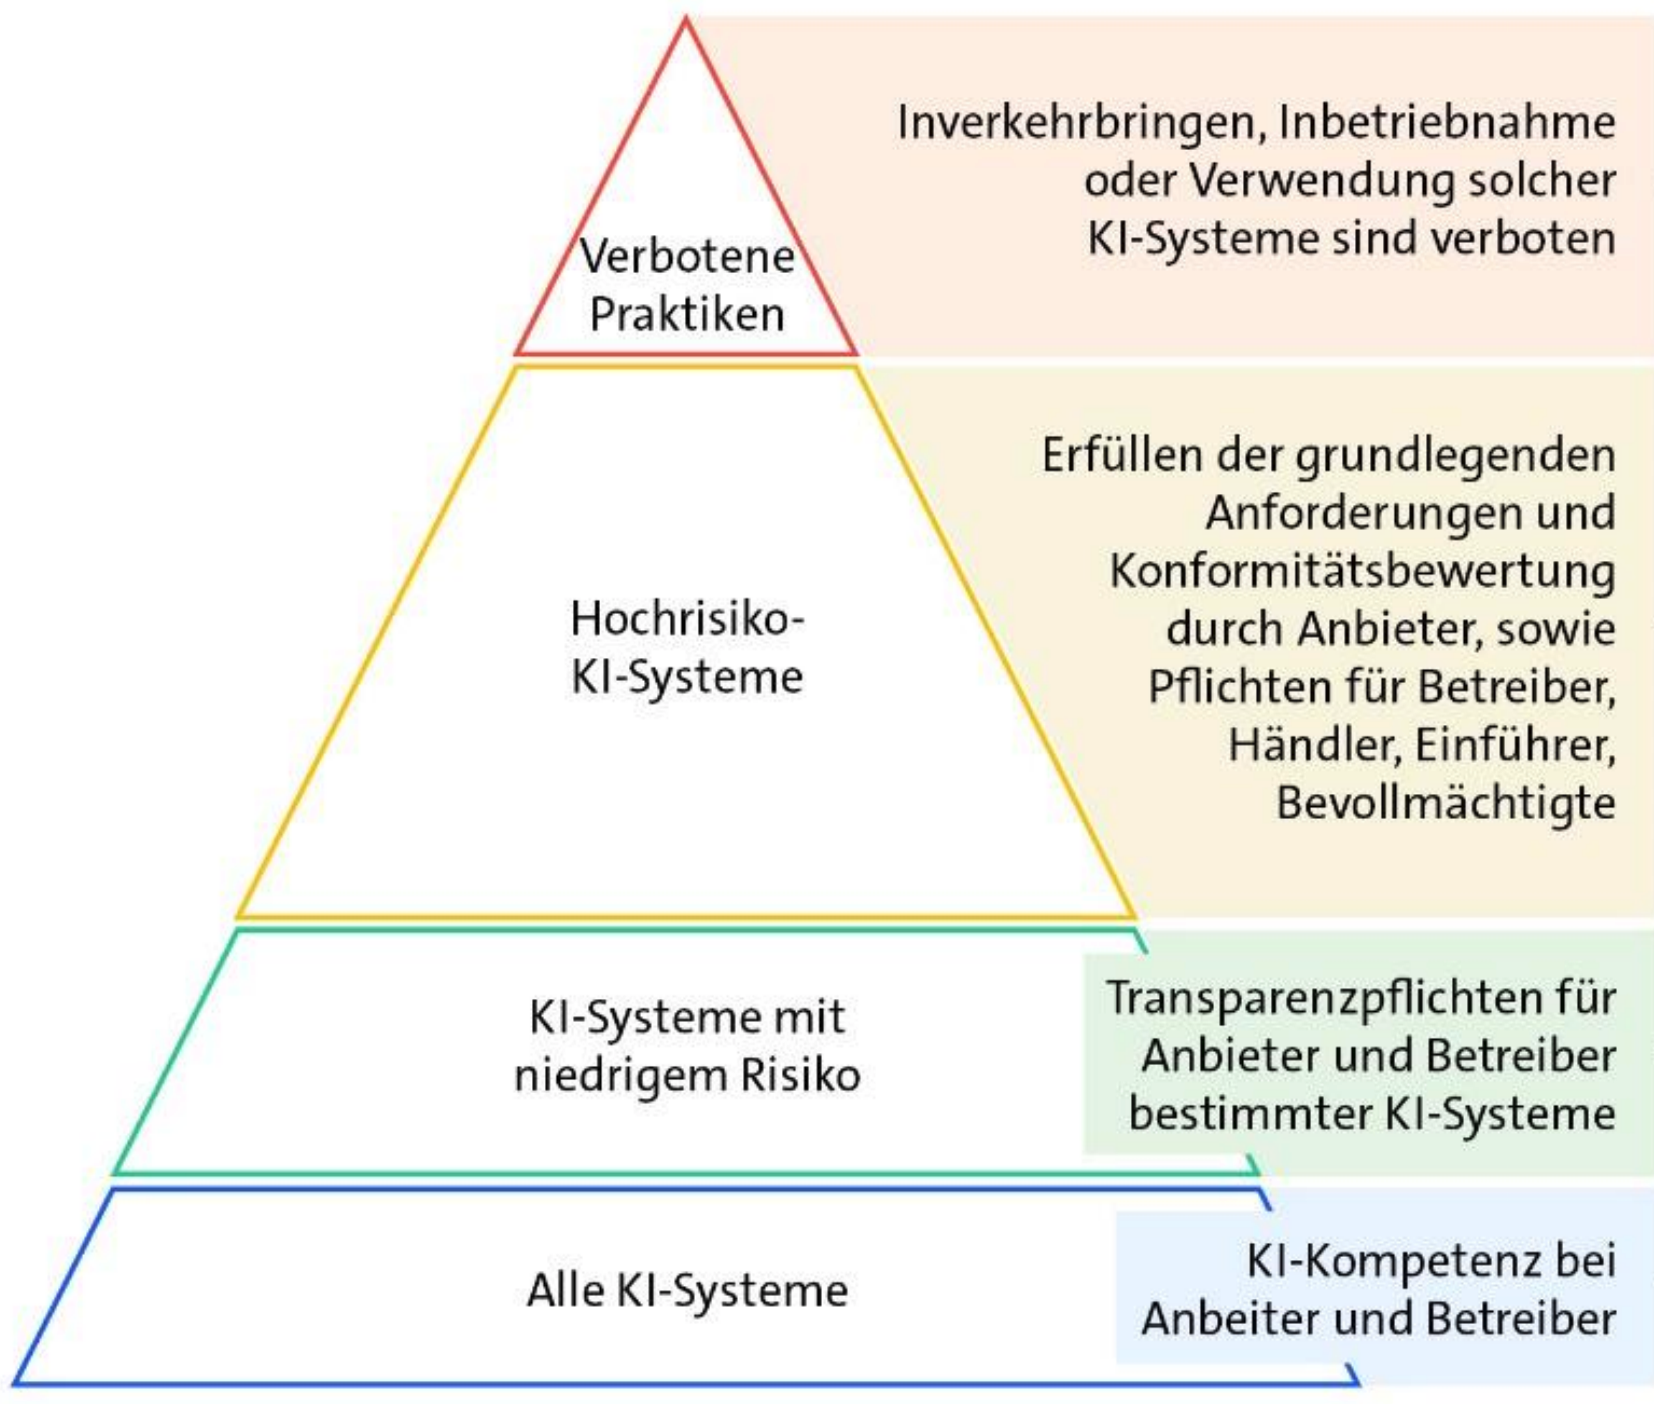
\includegraphics[width=0.8\textwidth]{images/bitcom_ki_vo_pyramide}
    \caption[Pisikopyramide KI-Systme]{Pisikopyramide KI-Systme\\Quelle: \cite{Bitkom2024Umsetzungsleitfaden}}
    \label{fig:bitcom_ki_vo_pyramide}
\end{figure}

Hinzukommen eventuell Verpflichtungen nach der DS-GVO, wenn in den Dokumenten personenbezogene Daten nach Artikel 4 DSG-VO, enthalten sein sollten.
Ebenso wie bei der Verletzung der KI-VO können auch hier hohe Bußgelder drohen.

\section{Reflexion der Arbeit}

Vor Beginn dieser Arbeit antizipierte wir bereits Schwierigkeiten bei der Bewertung von RAG-Systemen mittels RAGAS:
\begin{description}
    \item [\textbf{Kosten}] Die Kosten, die bei der Bewertung entstehen. %Welche Kosten, LLM Wartung etc.
    \item [\textbf{Zeitbedarf}] Die Dauer für die Durchführung der Bewertung. Die Bewertung kann schneller durchgeführt werden, wenn mehr Ressourcen zur Verfügung stehen.
    \item [\textbf{Implementierung}] Das Aufsetzen des zu testenden Systems. Dies beinhaltet eine eventuelle doppelte Speicherung der Daten und die für das Testen benötigten Aufrufe des LLMs. %Installation
    \item [\textbf{Aktualisierung}] Das System muss auf dem neuesten Stand gehalten werden, da sich dieses aktuelle Thema schnell entwickelt.
\end{description}


Während der Arbeit an dieser Bachelorarbeit gab es einige Herausforderungen und Erkenntnisse, die den Ablauf und die Ergebnisse beeinflusst haben. Hier sind einige Überlegungen zur Reflexion der Arbeit:

\begin{enumerate}

    \item{Dokumente}\\
    Im ersten Schritt, dem Sammeln der Dokumente und deren Aufbereitung, gab es einige Herausforderungen.
    Es standen nicht genügend originale Dokumente zur Verfügung, sodass synthetische Dokumente generiert werden mussten.
    Damit das LLM realistische Dokumente generieren kann, wurden die originalen Dokumente als Grundlage genutzt und neue Bereiche und und Projekte erfunden.

    \item{RAGs und RAGAS verstehen}\\
    Da es bereits Erfahrungen mit RAGs im betrieblichen Umfeld gab, war es einfach, die neuesten Entwicklungen zu verstehen.
    Die Einarbeitung in RAGAS und die Metriken war aufgrund der guten Dokumentation und der vorangegangenen Erfahrungen mit RAGs ebenfalls relativ einfach.
    Nicht nur die Verwendung der einzelnen Komponenten, sondern auch das Nutzen der einzelnen Metriken war einfach und gut umsetzbar.

    \item{Versuchsplan}\\
    Die Erstellung des Versuchsplans war eine große Herausforderung.
    Es mussten verschiedene Aspekte berücksichtigt werden, wie z. B. die Anzahl der Dokumente, die Art der Dokumente und die Modelle, die bewertet werden sollten.
    Zudem gab es eine Unvorhersehbarkeit der Dauer und Kosten der Versuche.
    Es konnte also erst nach den ersten Versuchen eine realistische Einschätzung der Dauer und Kosten gegeben werden.

    \item{Implementierung}\\
    Die grundlegende Implementierung von RAGAS war dank Langchain und der guten Dokumentation einfach.
    Durch die vielen Abhängigkeiten und die schnelle Weiterentwicklung von Python-Bibliotheken gab es jedoch einige Probleme, die die Implementierung erschwerten.
    So gab es ein Problem mit dem Paket LiteLLM; einen Fix gab es schon, aber dieser war noch nicht in Version 1.67.5 übernommen worden, weshalb dieser Fix eigens implementiert werden musste.
    Das System, welches implementiert wurde, war jedoch sehr hilfreich, da hier die Generierung der Testsets und die Bewertung der RAGs automatisiert im Hintergrund abliefen.
    Dies war besonders bei langlaufenden Versuchen wichtig, damit die Versuche nicht manuell gestartet werden mussten.

    \item{Versuche}\\
    Will man verhindern, dass eine definierte Grenze durch die Iteration überschritten wird, sollte man eine Durchsatzbegrenzung implementieren.
    Eine solche Durchsatzbegrenzung soll dann die zugrundeliegende Dienste und Resourcen schützen~\cite{BuiltinRateLimiter}.
    Der implementierte Durchsatzbegrenzer war nicht sehr ausgereift und war einer der Punkte, welche die Dauer der Versuche verlängert haben.
    Sowohl bei OpenAI als auch bei DeepSeek gab es Probleme mit der Durchsatzbegrenzungs-Implementierung, welche zu ungültigen Ergebnissen führten und das erneute Starten der Versuche notwendig machten.
    Auch die Auswahl der Hardware wurde während der Arbeit gewechselt, da zuerst auf einem Laptop gearbeitet wurde, welcher nicht die Leistung hatte, um die Versuche in einem angemessenen Zeitrahmen durchzuführen.
    Die 32 GB RAM wurden komplett ausgeschöpft und führten zum Absturz des Systems.
    Das finale System, ein M2 Ultra mit 192 GB RAM, konnte die Versuche in einem angemessenen Zeitrahmen durchführen und war auch für die zukünftige Nutzung praxistauglich.

    \item{Auswertung}\\
    Die Auswertung war aufgrund der vielen Daten und der manuellen Auswertung aufwendig; außerdem fielen Fehler während der manuellen Auswertung auf.
    Diese führten dazu, dass die Auswertung der Fragebögen und der Bewertungen länger dauerte und erneut ausgeführt werden musste.
    Einer der Fehler wurde auch durch die Intransparenz der Modellversionierung seitens OpenAI verursacht.
    Während des Versuchs für die Zuverlässigkeit der Bewertung wurde die Modellversion von GPT-4 geändert, was zu einer Abweichung der Ergebnisse führte und das erneute Durchführen der Versuche erforderte.

\end{enumerate}